\documentclass[a4paper]{article}

%% Language and font encodings
\usepackage[french]{babel}
\usepackage[utf8]{inputenc}
\usepackage[T1]{fontenc}

\usepackage{float}

\setlength{\parindent}{1em}
%\setlength{\parskip}{1ex plus 0.5ex minus 0.2ex}
\newcommand{\hsp}{\hspace{20pt}}
\newcommand{\HRule}{\rule{\linewidth}{0.5mm}}

\usepackage{algorithm}
\usepackage[noend]{algpseudocode}
\algnewcommand{\algorithmicand}{\textbf{ and }}
\algnewcommand{\algorithmicor}{\textbf{ or }}
\algnewcommand{\OR}{\algorithmicor}
\algnewcommand{\AND}{\algorithmicand}
\algnewcommand\algorithmicforeach{\textbf{for each}}
\algdef{S}[FOR]{ForEach}[1]{\algorithmicforeach\ #1\ \algorithmicdo}
\newcommand{\myfrac}[2]{\frac{\displaystyle {#1}}{\displaystyle {#2}}}

%% Sets page size and margins
\usepackage[a4paper,top=3cm,bottom=2cm,left=3cm,right=3cm,marginparwidth=1.75cm]{geometry}

%% Useful packages
\usepackage{amsmath}
\usepackage{amssymb}
\usepackage{graphicx}
\usepackage{subcaption}
\usepackage[colorinlistoftodos]{todonotes}
\usepackage[colorlinks=true, allcolors=blue]{hyperref}
\usepackage{graphicx}

\usepackage{enumitem}
\setitemize{label=\textbullet, font=\small}

%% equations
\usepackage{amsthm}
\usepackage[retainorgcmds]{IEEEtrantools}

%% Matlab
\usepackage[framed,numbered,autolinebreaks,useliterate]{mcode}

%% theorem and proposition
\newtheorem{prop}{Proposition}
\newtheorem*{prop*}{Proposition}
\newtheorem{thm}{Théorème}

\newenvironment{myproof}[1][\proofname]{\proof[#1]\mbox{}\\*}{\endproof}

%% references shortcuts (Arthur) 
\usepackage{suffix}
\renewcommand{\eqref}[1]{équation~\ref{#1}}
\newcommand{\algoref}[1]{algorithme~\ref{#1}}
\newcommand{\figref}[1]{figure~\ref{#1}}
\newcommand{\tabref}[1]{tableau~\ref{#1}}
\newcommand{\secref}[1]{section~\ref{#1}}
\newcommand{\probref}[1]{problème~\ref{#1}}
\newcommand{\propref}[1]{proposition~\ref{#1}}
\newcommand{\theoremref}[1]{théorème~\ref{#1}}
\newcommand{\chapref}[1]{chapitre~\ref{#1}}
\WithSuffix\newcommand\algoref*[1]{algorithme~\ref{#1} p.~\pageref{#1}}
\WithSuffix\newcommand\figref*[1]{figure~\ref{#1} p.~\pageref{#1}}
\WithSuffix\newcommand\eqref*[1]{équation~\ref{#1} p.~\pageref{#1}}
\WithSuffix\newcommand\tabref*[1]{tableau~\ref{#1} p.~\pageref{#1}}
\WithSuffix\newcommand\secref*[1]{section~\ref{#1} p.~\pageref{#1}}
\WithSuffix\newcommand\probref*[1]{problème~\ref{#1} p.~\pageref{#1}}
\WithSuffix\newcommand\propref*[1]{proposition~\ref{#1} p.~\pageref{#1}}
\WithSuffix\newcommand\chapref*[1]{chapitre~\ref{#1} p.~\pageref{#1}}

\usepackage[backend=biber,uniquename=init,giveninits=true,
             %% "et al" pour > deux auteurs, & pour exactement 2
             uniquelist=false,maxcitenames=2,mincitenames=1,maxbibnames=99,
             isbn=false,url=false,doi=false,bibstyle=numeric
]{biblatex}
\addbibresource{references.bib}

\begin{document}

\begin{titlepage}
  \begin{center}

      \makebox[0.5\textwidth][r]{%
        
\includegraphics[width=0.33\textwidth]{images/sorbonne.png}%
    }%

      \vspace{4cm}
    % Title
    \HRule \\[0.4cm]
    { \huge \bfseries BIMA\\[0.4cm] }

      \textsc{\LARGE Mini rapport TP5}\\[0.4cm]

    \HRule \\[0.8cm]

    % Author and supervisor
    \begin{minipage}{0.4\textwidth}
      \begin{flushleft} \large
        Kim-Anh Laura \textsc{Nguyen}\\
        \large
        Arij \textsc{Riabi}\\
        M1 DAC\\
        Promo 2018-2019 \\
      \end{flushleft}
    \end{minipage}
    \begin{minipage}{0.5\textwidth}
      \begin{flushright} \large
        \emph{Enseignant :} Dominique \textsc{Béréziat}\\
      \end{flushright}
    \end{minipage}

      \vspace{2cm}

  \end{center}
  %\end{sffamily}
\end{titlepage}
%\maketitle

\newpage

\section*{Exercice 1 - Comparaison de filtres discrets du 1er et du 2nd ordre}

\begin{enumerate}
    \item \textbf{Filtre de Sobel }

\begin{figure}[H]
\begin{lstlisting}
function [mod_seuille] = filtre_sobel(I, seuil)
    Gx = [1, 0, -1; 2, 0, -2; 1, 0, -1]; % filtre de Sobel en x
    Gy = [1, 2, 1; 0, 0, 0; -1, -2, -1]; % filtre de Sobel en y 
    Ix = convolution(I, Gx); % produit de convolution entre I et Gx 
    Iy = convolution(I, Gy); % produit de convolution entre I et Gy
    module = sqrt(Ix.^2 + Iy.^2); % calcul du module du gradient estime 
    % produit un filtre detecteur de contours du premier ordre
    mod_seuille = seuillerImage(module, seuil); 
end
\end{lstlisting}
\caption{Fonction \texttt{filtre\_sobel}}
\end{figure}

    \item \textbf{Filtre laplacien}

\begin{figure}[H]
\begin{lstlisting}
\centering
function [M] = filtre_laplacien(I,seuil)
    [n,m] = size(I);
    L = [0, 1, 0; 1, -4, 1; 0, 1, 0]; % masque laplacien 
    IL = convolution(I, L); % produit de convolution entre I et L
    
    % matrice n x m dont chaque pixel p vaut 255 s'il correspond a un contour
    % 0 autrement
    M = zeros(n,m);
    
    % determination des passages par 0 de IL
    for i=2:n-1
        for j=2:m-1
            sous_mat = IL(i-1:i+1, j-1:j+1);
            max_IL = max(max(sous_mat));
            min_IL = min(min(sous_mat));
    
            if ((max_IL > 0) && (min_IL < 0) && ((max_IL -min_IL) > seuil))
                M(i,j) = 1;
            end
        end
    end
end
\end{lstlisting}
\caption{Fonction \texttt{filtre\_laplacien}}
\end{figure}

    \item \textbf{Comparaison des deux filtres}

La \figref{fig:application-filtres} contient les images obtenues avec chaque
        filtre détecteur de contours sur l'image \texttt{lena.gif}
        (\figref{subfig:lena}). \\

On remarque que le filtre de Sobel (\figref{subfig:lena-sobel}) détecte les
        contours fins. En revanche, le masque laplacien
        (\figref{subfig:lena-laplacien}) génère des contours épais et est
        sensible au bruit (les hautes fréquences correspondant à
        l'arrière-plan). Cela est dû à la double dérivation, qui amplifie
        davantage le bruit, ainsi qu'à l'erreur
        de quantification, liée au fait que l'on traite une fonction entière et
        discrète.

\begin{figure}[H]
    \centering
    \begin{subfigure}[c]{0.3\textwidth}
        \centering
        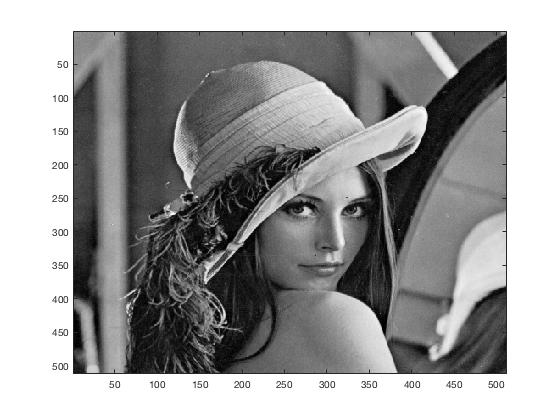
\includegraphics[width=\textwidth]{images/lena.png}
        \caption{Image originale} 
    \label{subfig:lena}
    \end{subfigure}
    \hspace{0.5cm}
    \begin{subfigure}[c]{0.3\textwidth}
        \centering
        
\includegraphics[width=\textwidth]{images/lena_sobel.png}
        \caption{Filtre détecteur de contours du premier ordre (seuil à 70)}
    \label{subfig:lena-sobel}
    \end{subfigure}
    \hspace{0.5cm}
    \begin{subfigure}[c]{0.3\textwidth}
        \centering
        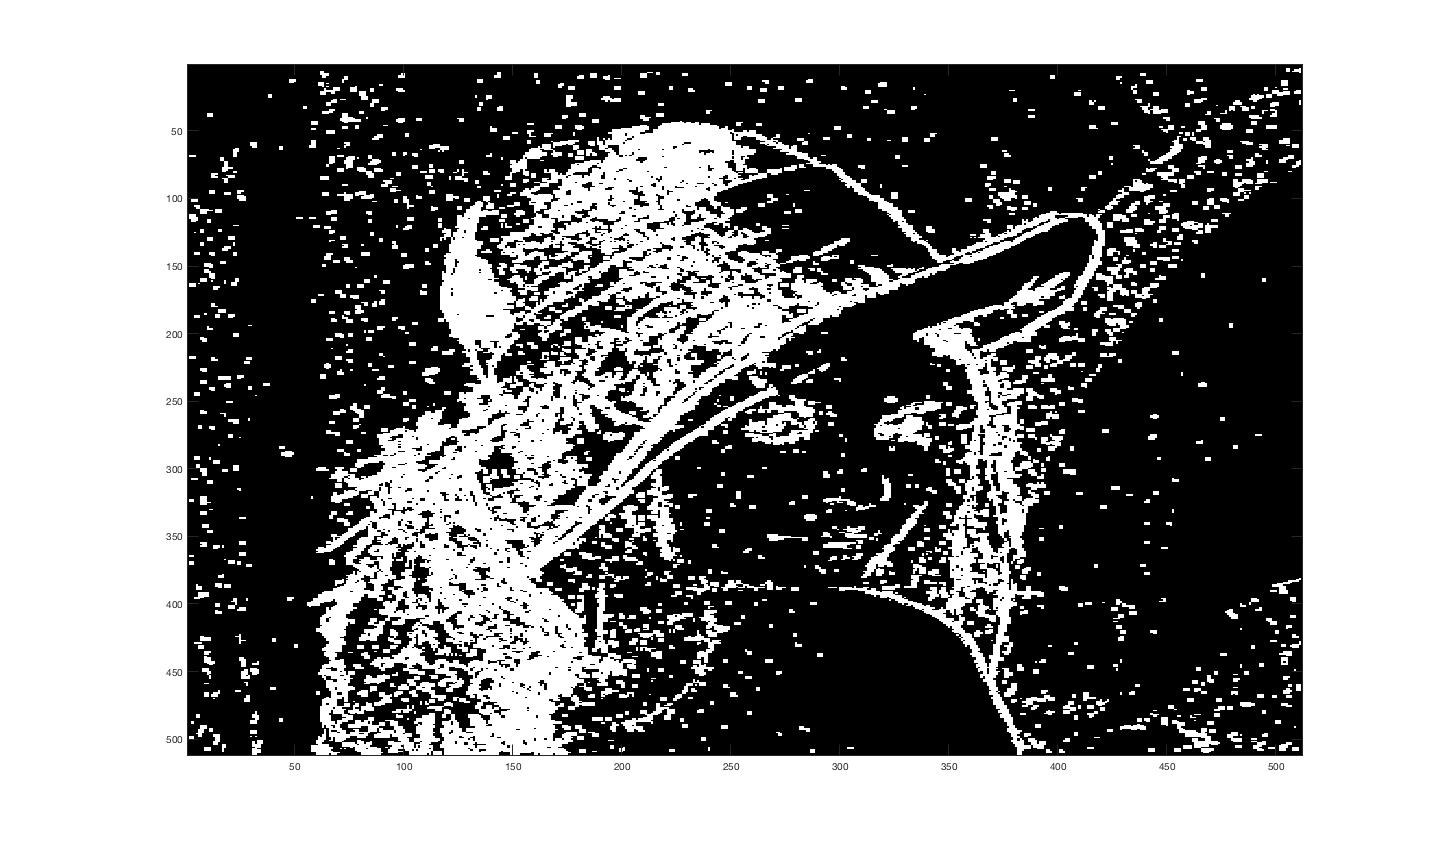
\includegraphics[width=1.5\textwidth]{images/lena_laplacien.png}
        \caption{Filtre détecteur de contours du second ordre (seuil à 70)}
    \label{subfig:lena-laplacien}
    \end{subfigure}

    \caption{Application des filtres détecteur de contours du premier et du
    second ordre sur l'image \texttt{lena.gif}}
    \label{fig:application-filtres}
\end{figure}

\end{enumerate}

\section*{Exercice 2 - Suppression de non maxima}

\begin{figure}[H]
    \centering
    \begin{subfigure}[c]{0.46\textwidth}
        \centering
        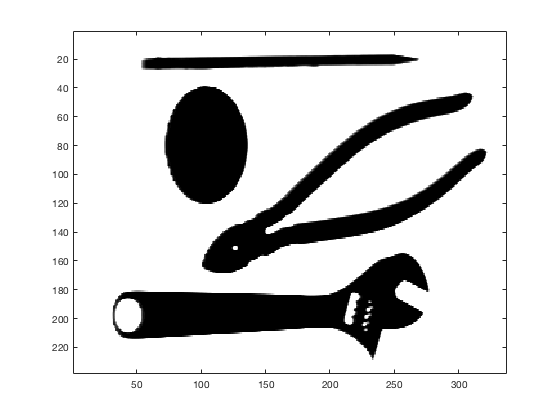
\includegraphics[width=\textwidth]{images/tools.png}
    \end{subfigure}
    \begin{subfigure}[c]{0.46\textwidth}
        \centering
        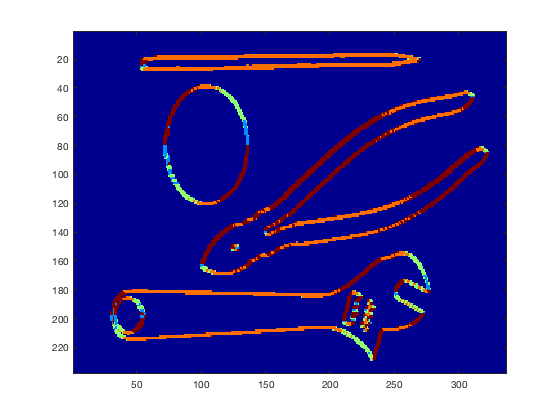
\includegraphics[width=\textwidth]{images/tools_orientation.png}
    \end{subfigure}
    \caption{Image \texttt{tools.gif} et image de l'orientation des gradients
    associés}
    \label{fig:tools-orientation}
\end{figure}

\begin{figure}[H]
\centering
\begin{lstlisting}
function [new_Ig] = nms(Ig,Ior)
    % Ig : image du module du gradient
    % Ior : image de l'orientation des gradients 
    % renvoie une image du module du gradient ou seuls
    % les extrema locaux sont conserves
    
    [n,m] = size(Ig);
    zeros_c = zeros(n,1); % colonne de zeros 
    zeros_l = zeros(1, m+2); % ligne de zeros

    % Ig2 : matrice Ig dans laquelle on rajoute 
    % de part et d'autre 2 lignes et 2 colonnes de zeros
    Ig2 = [zeros_c Ig zeros_c];
    Ig2 = [zeros_l; Ig2; zeros_l];
    new_Ig = zeros(n,m);
    
    for i=2:n+1
        for j=2:m+1
            or = Ior(i-1,j-1);
            v = Ig2(i,j);
            if or == 1 % ouest, est
                v1 = Ig2(i,j-1);
                v2 = Ig2(i,j+1);
            elseif or == 2 % nord-est, sud-ouest
                v1 = Ig2(i-1,j+1);
                v2 = Ig2(i+1,j-1);
            elseif or == 3 % nord, sud
                v1 = Ig2(i-1,j);
                v2 = Ig2(i+1,j);
            elseif or == 4 % nord-ouest, sud-est
                v1 = Ig2(i-1,j-1);
                v2 = Ig2(i+1,j+1);
            else
                continue
            end
            
            if (v > v1) && (v > v2)
                new_Ig(i-1,j-1) = 255;
            end
        end
    end
end
\end{lstlisting}
\caption{Fonction \texttt{nms}}
\end{figure}

Comme l'on met à zéro la norme du gradient pour les pixels non maxima locaux, on
obtient donc des contours d'épaisseur 1 pixel.

\begin{figure}[H]
    \centering
    \begin{subfigure}[c]{0.46\textwidth}
        \centering
        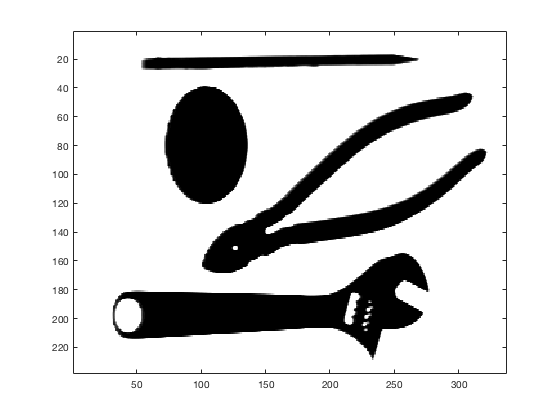
\includegraphics[width=\textwidth]{images/tools.png}
    \end{subfigure}
    \begin{subfigure}[c]{0.46\textwidth}
        \centering
        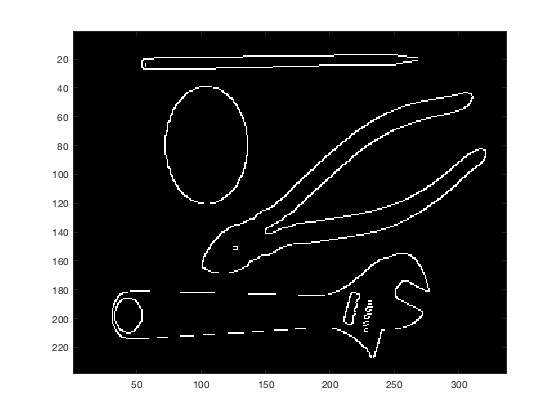
\includegraphics[width=\textwidth]{images/tools_nms.png}
    \end{subfigure}
    \caption{Image \texttt{tools.gif} et image du module du gradient avec
    suppression de non maxima, sans lissage gaussien}
    \label{fig:tools-nms}
\end{figure}

\begin{figure}[H]
    \centering
    \begin{subfigure}[c]{0.46\textwidth}
        \centering
        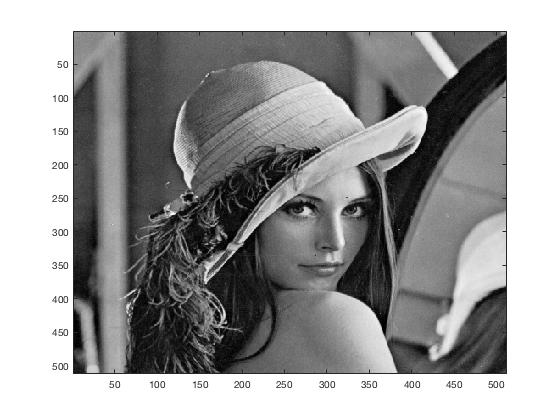
\includegraphics[width=\textwidth]{images/lena.png}
    \end{subfigure}
    \begin{subfigure}[c]{0.46\textwidth}
        \centering
        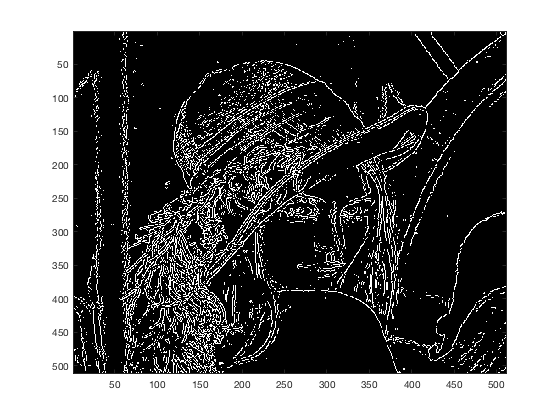
\includegraphics[width=\textwidth]{images/lena_nms.png}
    \end{subfigure}
    \caption{Image \texttt{lena.gif} et image du module du gradient avec
    suppression de non maxima, sans lissage gaussien}
    \label{fig:tools-nms}
\end{figure}

\begin{figure}[H]
    \centering
    \begin{subfigure}[c]{0.46\textwidth}
        \centering
        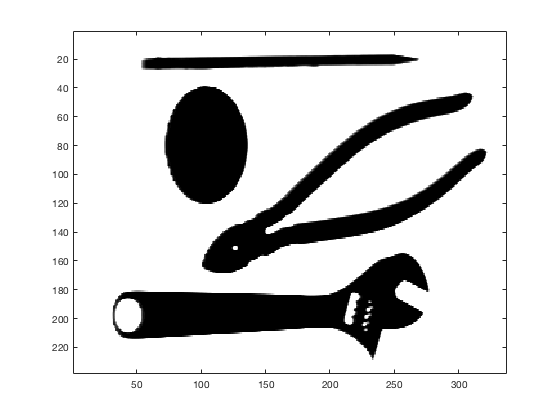
\includegraphics[width=\textwidth]{images/tools.png}
    \end{subfigure}
    \begin{subfigure}[c]{0.46\textwidth}
        \centering
        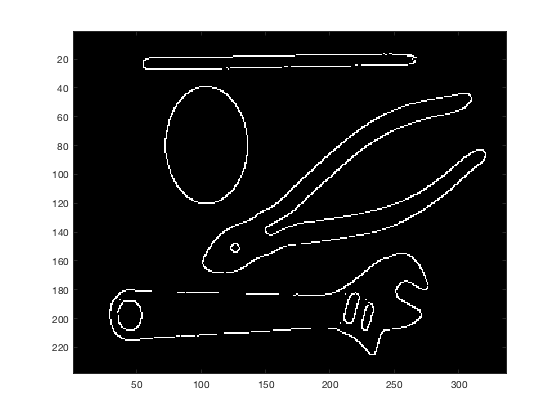
\includegraphics[width=\textwidth]{images/tools_nms_gauss.png}
    \end{subfigure}
    \caption{Image \texttt{tools.gif} et image du module du gradient avec
    suppression de non maxima, et lissage gaussien ($\sigma = 3$)}
    \label{fig:tools-nms-gauss}
\end{figure}

\begin{figure}[H]
    \centering
    \begin{subfigure}[c]{0.46\textwidth}
        \centering
        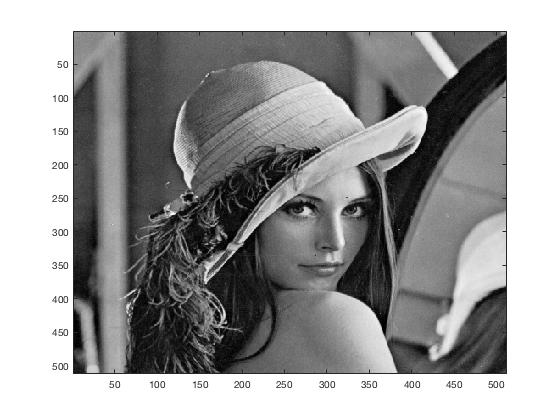
\includegraphics[width=\textwidth]{images/lena.png}
    \end{subfigure}
    \begin{subfigure}[c]{0.46\textwidth}
        \centering
        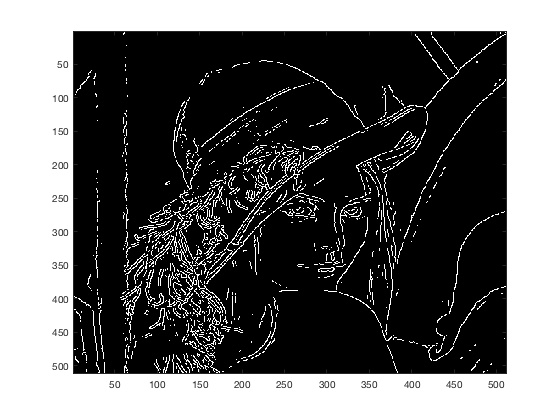
\includegraphics[width=\textwidth]{images/lena_nms_gauss1.png}
    \end{subfigure}
    \caption{Image \texttt{lena.gif} et image du module du gradient avec
    suppression de non maxima, et lissage gaussien ($\sigma = 1$)}
    \label{fig:lena-nms-gauss}
\end{figure}

On remarque sur les figures \ref{fig:tools-nms-gauss} et
\ref{fig:lena-nms-gauss} qu'un lissage gaussien (à $\sigma=3$ pour
\texttt{tools.gif} et $\sigma=1$ pour \texttt{lena.gif}) appliqué avant la
différentiation permet de réduire le bruit : les variations locales sont
filtrées et les contours dominants restent.

\begin{figure}[H]
    \centering
    \begin{subfigure}[c]{0.3\textwidth}
        \centering
        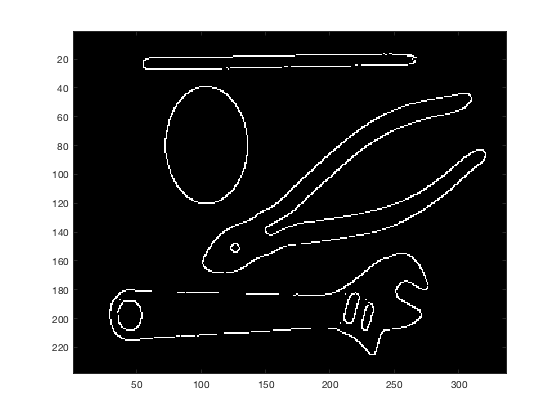
\includegraphics[width=\textwidth]{images/tools_nms_gauss.png}
        \caption{$\sigma=3$}
    \end{subfigure}
    \begin{subfigure}[c]{0.3\textwidth}
        \centering
        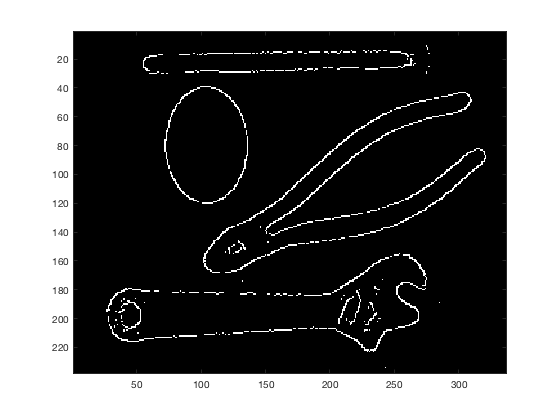
\includegraphics[width=\textwidth]{images/tools_nms_gauss5.png}
        \caption{$\sigma=5$}
    \end{subfigure}
    \begin{subfigure}[c]{0.3\textwidth}
        \centering
        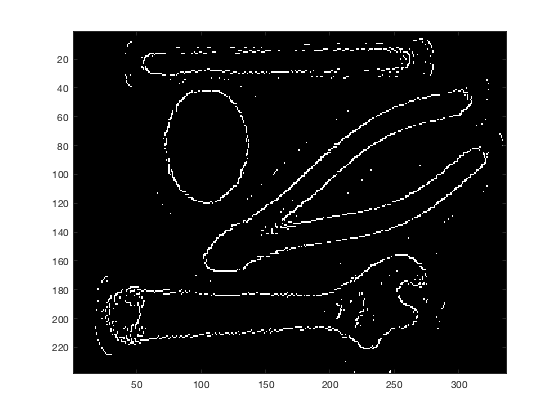
\includegraphics[width=\textwidth]{images/tools_nms_gauss7.png}
        \caption{$\sigma=7$}
    \end{subfigure}

    \caption{Images du module du gradient de \texttt{tools.gif} avec
    suppression de non maxima, et lissage gaussien}
    \label{fig:tools-nms-gauss-var}
\end{figure}

\begin{figure}[H]
    \centering
    \begin{subfigure}[c]{0.3\textwidth}
        \centering
        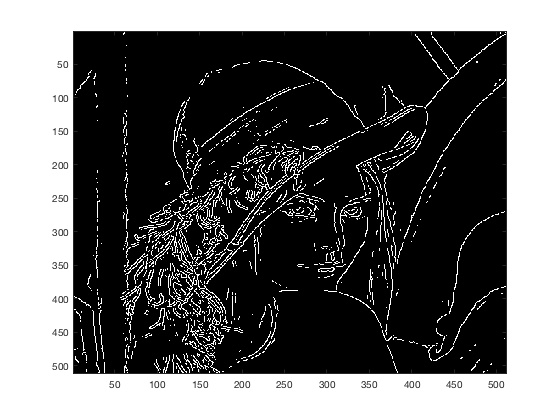
\includegraphics[width=\textwidth]{images/lena_nms_gauss1.png}
        \caption{$\sigma=1$}
    \end{subfigure}
    \begin{subfigure}[c]{0.3\textwidth}
        \centering
        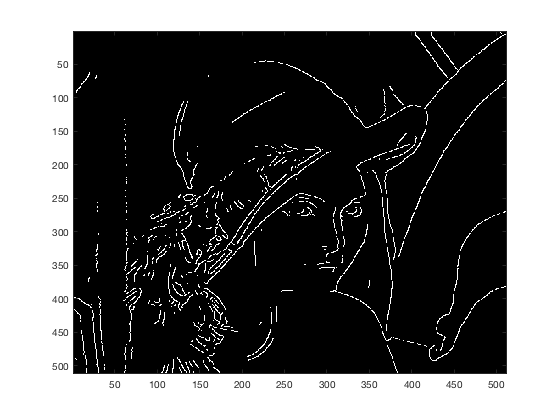
\includegraphics[width=\textwidth]{images/lena_nms_gauss2.png}
        \caption{$\sigma=2$}
    \end{subfigure}
    \begin{subfigure}[c]{0.3\textwidth}
        \centering
        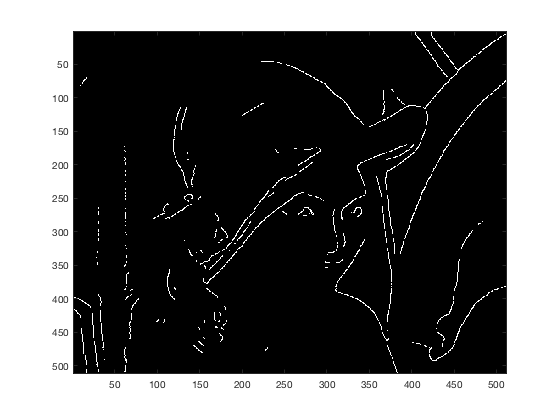
\includegraphics[width=\textwidth]{images/lena_nms_gauss3.png}
        \caption{$\sigma=3$}
    \end{subfigure}

    \caption{Images du module du gradient de \texttt{lena.gif} avec
    suppression de non maxima, et lissage gaussien}
    \label{fig:lena-nms-gauss-var}
\end{figure}

\section*{Exercice 3 - Influence du lissage dans la détection de contours}

\begin{figure}[H]
    \centering
    \begin{subfigure}[c]{0.46\textwidth}
        \centering
        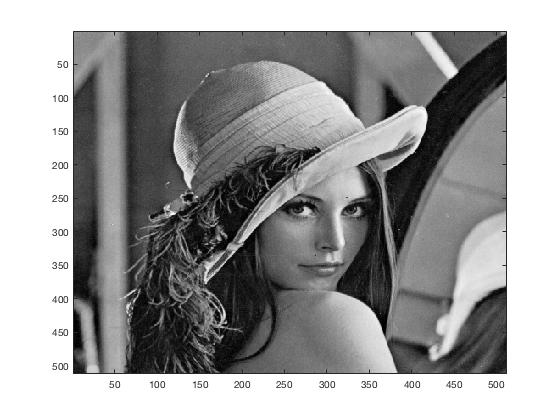
\includegraphics[width=\textwidth]{images/lena.png}
    \end{subfigure}
    \begin{subfigure}[c]{0.46\textwidth}
        \centering
        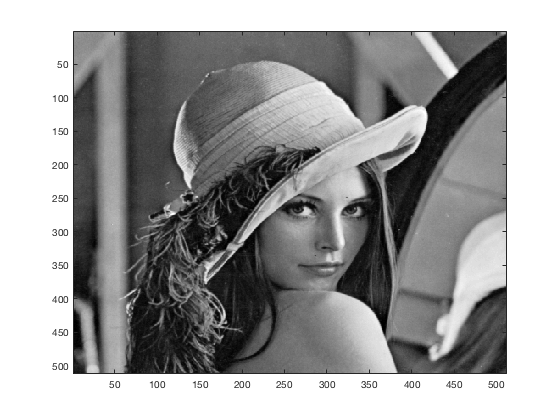
\includegraphics[width=\textwidth]{images/lena_lissage.png}
    \end{subfigure}
    \caption{Image \texttt{lena.gif} originale et lissage gaussien avec
    $\sigma=0.5$}
    \label{fig:lena-lissage}
\end{figure}

\begin{figure}[H]
    \centering
    \begin{subfigure}[c]{0.46\textwidth}
        \centering
        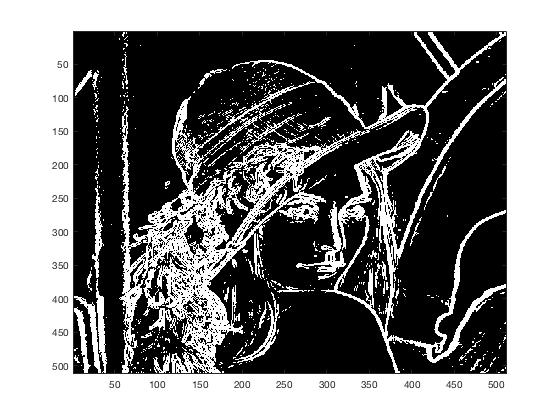
\includegraphics[width=\textwidth]{images/lena_gauss_sobel.png}
    \end{subfigure}
    \begin{subfigure}[c]{0.46\textwidth}
        \centering
        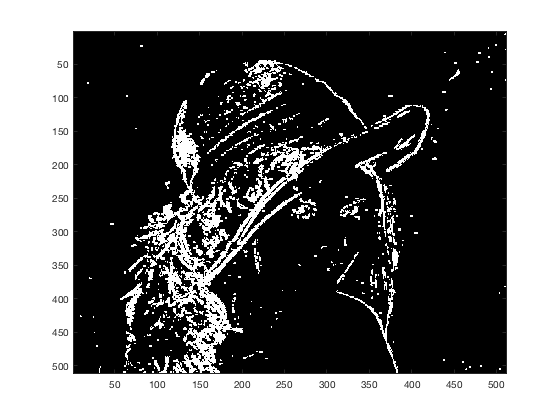
\includegraphics[width=\textwidth]{images/lena_gauss_laplacien.png}
    \end{subfigure}
    \caption{Application des filtres de Sobel et laplacien à l'image
    \texttt{lena.gif} lissée ($\sigma=0.5$)}
    \label{fig:lena-lissage}
\end{figure}

\begin{figure}[H]
    \centering
    \begin{subfigure}[c]{0.46\textwidth}
        \centering
        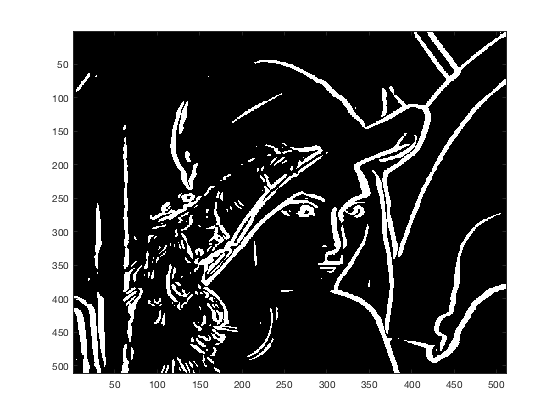
\includegraphics[width=\textwidth]{images/lena_gauss_sobel2.png}
    \end{subfigure}
    \begin{subfigure}[c]{0.46\textwidth}
        \centering
        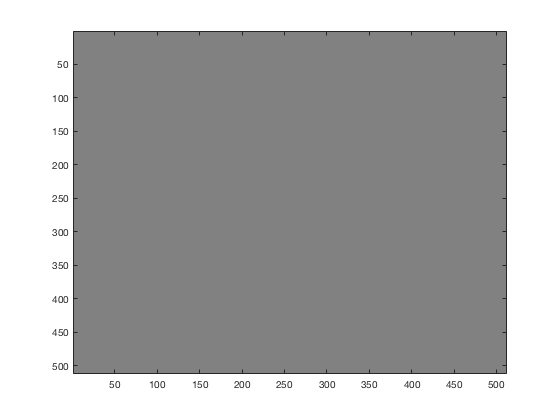
\includegraphics[width=\textwidth]{images/lena_gauss_laplacien2.png}
    \end{subfigure}
    \caption{Application des filtres de Sobel et laplacien à l'image
    \texttt{lena.gif} lissée ($\sigma=2$)}
    \label{fig:lena-lissage}
\end{figure}

\begin{figure}[H]
    \centering
    \begin{subfigure}[c]{0.46\textwidth}
        \centering
        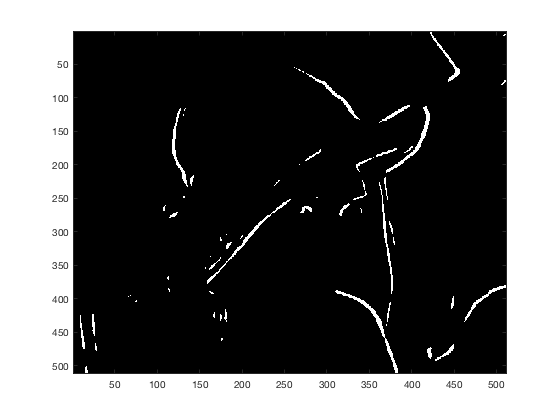
\includegraphics[width=\textwidth]{images/lena_gauss_sobel3.png}
    \end{subfigure}
    \begin{subfigure}[c]{0.46\textwidth}
        \centering
        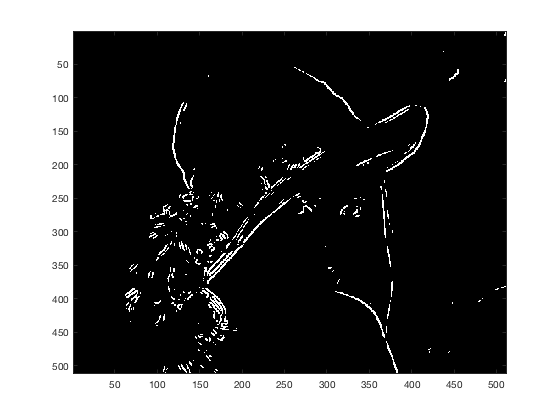
\includegraphics[width=\textwidth]{images/lena_gauss_laplacien3.png}
    \end{subfigure}
    \caption{Application des filtres de Sobel et laplacien à l'image
    \texttt{lena.gif} lissée ($\sigma=2$) avec des seuils respectifs de 150 et
    10}
    \label{fig:lena-lissage}
\end{figure}

%La \figref{fig:filtrage-mandrill1} (resp. \ref{fig:filtrage-lena1}) montrent les
%étapes du filtrage passe-bas de l'image \ref{subfig:mandrill1} (resp.
%\ref{subfig:lena1}).
%
%\begin{figure}[H]
%    \centering
%    \begin{subfigure}[c]{0.46\textwidth}
%        \centering
%        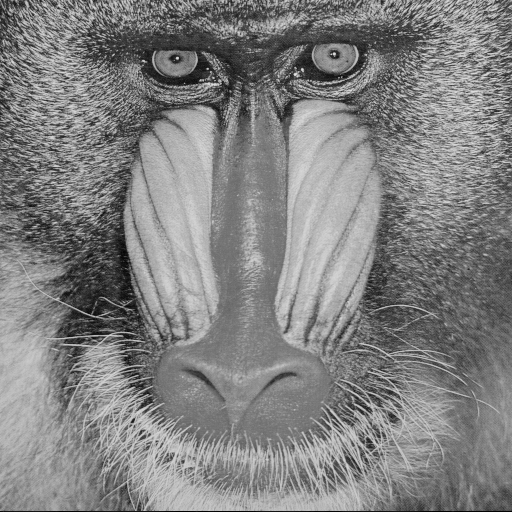
\includegraphics[width=\textwidth]{images/mandrill.png}
%        \caption{Image originale} 
%    \label{subfig:mandrill1}
%    \end{subfigure}
%    \begin{subfigure}[c]{0.46\textwidth}
%        \centering
%        \includegraphics[width=\textwidth]{images/mandrill_FT1.png}
%        \caption{Module centré de la transformée de Fourier de l'image}
%    \label{subfig:mandrill-FT1}
%    \end{subfigure}
%
%    \begin{subfigure}[c]{0.46\textwidth}
%        \centering
%        \includegraphics[width=\textwidth]{images/mandrill_FT_filtre1.png}
%        \caption{Module centré de la transformée de Fourier filtrée} 
%        \label{subfig:mandrill-FT-filtre1}
%    \end{subfigure}
%    \begin{subfigure}[c]{0.46\textwidth}
%        \centering
%        \includegraphics[width=\textwidth]{images/mandrill_filtre1.png}
%        \caption{Image filtrée}
%    \label{subfig:mandrill-filtre1}
%    \end{subfigure}
%
%    \caption{Étapes du filtrage passe-bas de l'image \texttt{mandrill.png} avec $f_c = 30$}
%    \label{fig:filtrage-mandrill1}
%\end{figure}
%
%\begin{figure}[H]
%    \centering
%    \begin{subfigure}[c]{0.46\textwidth}
%        \centering
%        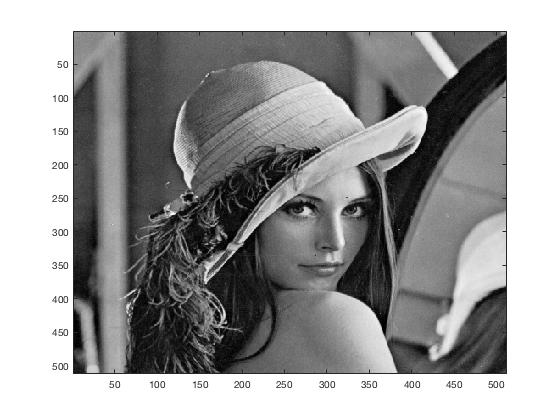
\includegraphics[width=\textwidth]{images/lena.png}
%        \caption{Image originale} 
%    \label{subfig:lena1}
%    \end{subfigure}
%    \begin{subfigure}[c]{0.46\textwidth}
%        \centering
%        \includegraphics[width=\textwidth]{images/lena_FT1.png}
%        \caption{Module centré de la transformée de Fourier de l'image}
%    \label{subfig:lena-FT1}
%    \end{subfigure}
%
%    \begin{subfigure}[c]{0.46\textwidth}
%        \centering
%        \includegraphics[width=\textwidth]{images/lena_FT_filtre1.png}
%        \caption{Module centré de la transformée de Fourier filtrée} 
%    \label{subfig:lena-FT-filtre1}
%    \end{subfigure}
%    \begin{subfigure}[c]{0.46\textwidth}
%        \centering
%        \includegraphics[width=\textwidth]{images/lena_filtre1.png}
%        \caption{Image filtrée}
%    \label{subfig:lena-filtre1}
%    \end{subfigure}
%
%    \caption{Étapes du filtrage passe-bas de l'image \texttt{lena.png} de
%    fréquence de coupure $f_c = 30$}
%    \label{fig:filtrage-lena1}
%\end{figure}
%
%\begin{figure}[H]
%    \centering
%    \begin{subfigure}[c]{0.46\textwidth}
%        \centering
%        \includegraphics[width=\textwidth]{images/lena_filtre2.png}
%        \caption{Image \texttt{lena.jpg} filtrée} 
%    \label{subfig:lena-filtre-2}
%    \end{subfigure}
%    \begin{subfigure}[c]{0.46\textwidth}
%        \centering
%        \includegraphics[width=\textwidth]{images/mandrill_filtre2.png}
%        \caption{Image \texttt{mandrill.png} filtrée} 
%    \label{subfig:mandrill-filtre2}
%    \end{subfigure}
%    \caption{Images filtrées avec un filtre passe-bas de fréquence de coupure
%    $f_c$ = 10}
%    \label{fig:filtrage-lena1}
%\end{figure}
%
%
%Lorsque l'on diminue la fréquence de coupure $f_c$, les changements brusques
%d'intensité sont atténués et l'image reconstruite présente plus de flou sur le
%contour. \\
%
%Ce type de filtrage fréquentiel est utilisé :
%\begin{itemize}
%    \item comme filtre anti-repliement dans la numérisation des signaux
%    \item pour filtrer le bruit.
%\end{itemize}
%
%\section*{Exercice 2 - Filtrage linéaire}
%
%Pour un filtre de taille $d$, on ajoute de part et d'autre de l'image $d-1$
%lignes et $d-1$ colonnes de zéros.
%
%La fonction \texttt{convolution} est testée sur l'image \texttt{barbara.png}
%avec les filtres moyenneurs $3 \times 3$, $5 \times 5$, $7 \times 7$. Les images
%résultantes sont présentées dans la \figref{fig:filtre-moy}.
%
%\begin{figure}[H]
%    \centering
%    \begin{subfigure}[c]{0.3\textwidth}
%        \centering
%        \includegraphics[width=\textwidth]{images/filtre_moy_3.png}
%        \caption{Application du filtre moyenneur $3 \times 3$} 
%        \label{subfig:filtre-moy-3}
%    \end{subfigure}
%    \begin{subfigure}[c]{0.3\textwidth}
%        \centering
%        \includegraphics[width=\textwidth]{images/filtre_moy_5.png}
%        \caption{Application du filtre moyenneur $5 \times 5$} 
%        \label{subfig:filtre-moy-5}
%    \end{subfigure}
%    \begin{subfigure}[c]{0.3\textwidth}
%        \centering
%        \includegraphics[width=\textwidth]{images/filtre_moy_7.png}
%        \caption{Application du filtre moyenneur $7 \times 7$} 
%        \label{subfig:filtre-moy-7}
%    \end{subfigure}
%    \caption{Application de filtres moyenneurs sur l'image \texttt{barbara.png}}
%    \label{fig:filtre-moy}
%\end{figure}
%
%On constate que plus la taille du filtre est grande, plus le lissage est important et
%plus l'image filtrée perd en détails par rapport à l'image originale.\\
%
%Les fonctions de transfert correspondants à ces filtres sont contenues dans la
%\figref{fig:transfert-moy}.
%
%\begin{figure}[H]
%    \centering
%    \begin{subfigure}[c]{0.3\textwidth}
%        \centering
%        \includegraphics[width=\textwidth]{images/transfert_moy_7.png}
%        \caption{Fonction de transfert du filtre moyenneur $3 \times 3$} 
%        \label{subfig:transfert-moy-3}
%    \end{subfigure}
%    \begin{subfigure}[c]{0.3\textwidth}
%        \centering
%        \includegraphics[width=\textwidth]{images/transfert_moy_5.png}
%        \caption{Fonction de transfert du filtre moyenneur $5 \times 5$} 
%        \label{subfig:transfert-moy-5}
%    \end{subfigure}
%    \begin{subfigure}[c]{0.3\textwidth}
%        \centering
%        \includegraphics[width=\textwidth]{images/transfert_moy_7.png}
%        \caption{Fonction de transfert du filtre moyenneur $7 \times 7$} 
%        \label{subfig:transfert-moy-7}
%    \end{subfigure}
%    \caption{Fonction de transfert des filtres moyenneurs}
%    \label{fig:transfert-moy}
%\end{figure}
%
%La fonction de transfert d'un filtre moyenneur de taille $d$ est :
%
%$$ H(f) = d \cdot sinc(\pi fa)$$
%
%Le filtre moyenneur est un filtre passe-bas qui a l'inconvénient d'être très peu
%sélectif : si l'on augmente $d$, on réduit encore plus les hautes fréquences
%mais on altère aussi les basses fréquences. Il n'est donc pas idéal.
%
%\section*{Exercice 3 - Filtrage anti-aliasing}
%
%Le sous-échantillonnage introduit nécessairement des effets d'aliasing. Afin de
%limiter ce problème, on effectue donc un filtrage passe-bas avant de
%sous-échantillonner. La \figref{fig:filtrage-anti-aliasing} contient l'image
%résultante après filtrage et sous-échantillonnage de l'image
%\texttt{barbara.png} (\ref{subfig:barbara-avec-anti-aliasing}), et celle générée
%par un sous-échantillonnage brutal (\ref{subfig:barbara-sans-anti-aliasing}).
%
%\begin{figure}[H]
%    \centering
%    \begin{subfigure}[c]{0.46\textwidth}
%        \centering
%        \includegraphics[width=\textwidth]{images/barbara_sous_echantillonage_avec_anti_aliassing.png}
%        \caption{Sous-échantillonnage avec anti-aliasing} 
%        \label{subfig:barbara-avec-anti-aliasing}
%    \end{subfigure}
%    \begin{subfigure}[c]{0.46\textwidth}
%        \centering
%        \includegraphics[width=\textwidth]{images/barbara_sous_echantillonage_sans_anti_aliassing.png}
%        \caption{Sous-échantillonnage sans anti-aliasing} 
%        \label{subfig:barbara-sans-anti-aliasing}
%    \end{subfigure}
%    \caption{Comparaison entre sous-échantillonnage avec anti-aliasing et
%    sous-échantillonnage sans anti-aliasing de l'image \texttt{barbara.png}}
%    \label{fig:filtrage-anti-aliasing}
%\end{figure}
%
%Lorsque la condition de Shannon n'est pas respectée, on est en situation de
%sous-échantillonnage. Il peut alors se produire un repliement de spectre : il y
%a perte d'information, on ne peut pas reconstruire l'image de départ et l'on se
%retrouve avec un effet de crénelage.
%
%Afin de pallier à ce problème, on effectue un filtrage anti-aliasing
%préalablement au sous-échantillonnage. Les hautes fréquences, i.e. tous les
%petits détails de l'image, seront bloquées (filtre passe-bas). Les zones de
%haute fréquence seront donc lissées et paraîtront légèrement floues. Ce filtre
%améliore donc la qualité de l'image.
%
%\begin{figure}[H]
%    \centering
%    \begin{subfigure}[c]{0.46\textwidth}
%        \centering
%        \includegraphics[width=\textwidth]{images/mandrill_sous_echantillonage_avec_anti_aliassing.png}
%        \caption{Sous-échantillonnage avec anti-aliasing} 
%        \label{subfig:mandrill-avec-anti-aliasing}
%    \end{subfigure}
%    \begin{subfigure}[c]{0.46\textwidth}
%        \centering
%        \includegraphics[width=\textwidth]{images/mandrill_sous_echantillonage_sans_anti_aliassing.png}
%        \caption{Sous-échantillonnage sans anti-aliasing} 
%        \label{subfig:mandrill-sans-anti-aliasing}
%    \end{subfigure}
%    \caption{Comparaison entre sous-échantillonnage avec anti-aliasing et
%    sous-échantillonnage sans anti-aliasing de l'image \texttt{mandrill.png}}
%    \label{fig:filtrage-anti-aliasing}
%\end{figure}
%
%\section*{Exercice 4 - Éclatement d'une image couleur}
%
%\begin{figure}[H]
%    \centering
%    \begin{subfigure}[c]{0.46\textwidth}
%        \centering
%        \includegraphics[width=\textwidth]{images/clown.png}
%        \caption{Image \texttt{clown.bmp}} 
%        \label{subfig:clown}
%    \end{subfigure}
%    \begin{subfigure}[c]{0.46\textwidth}
%        \centering
%        \includegraphics[width=\textwidth]{images/clown_lumi.png}
%        \caption{Image \texttt{clown\_lumi.bmp}} 
%        \label{subfig:clown_lumi}
%    \end{subfigure}
%    \caption{Visualisation des images \texttt{clown.bmp} et
%    \texttt{clown\_lumi.bmp}}
%    \label{fig:clowns}
%\end{figure}
%
%L'image \texttt{clown.bmp} (\figref{subfig:clown}) est en couleur (R,G,B) : il
%est représenté par un tableau à 3 dimensions. L'image \texttt{clown\_lumi.bmp}
%(\figref{subfig:clown_lumi}) est en noir et blanc.
%
%La première image est donc trois fois plus grande que la seconde.
%
%L’image I1 (\figref{subfig:clown}) possède les trois canaux R, G et B, qui
%représentent l’image dans chacune des couleurs Rouge Vert et Bleu.
%
%\begin{figure}[H]
%    \centering
%    \begin{subfigure}[c]{0.3\textwidth}
%        \centering
%        \includegraphics[width=\textwidth]{images/IR.png}
%        \caption{Composante rouge} 
%        \label{subfig:IR}
%    \end{subfigure}
%    \begin{subfigure}[c]{0.3\textwidth}
%        \centering
%        \includegraphics[width=\textwidth]{images/IV.png}
%        \caption{Composante verte} 
%        \label{subfig:IV}
%    \end{subfigure}
%    \begin{subfigure}[c]{0.3\textwidth}
%        \centering
%        \includegraphics[width=\textwidth]{images/IB.png}
%        \caption{Composante bleue} 
%        \label{subfig:IB}
%    \end{subfigure}
%    \caption{Composantes rouge, verte, et bleue de l'image \texttt{clown.bmp}}
%    \label{fig:composantes}
%\end{figure}
%
%\begin{figure}[H]
%	\center 
%	\includegraphics[width=0.5\textwidth]{images/Question3RBG.png}
%    \caption{Combinaison RBG}
%    \label{fig:RBG}
%\end{figure}
%
%L'image contenue dans la \figref{fig:RBG} représente une combinaison RBG
%(échange entre les plans vert et bleu). \\
%
%On souhaite voir le plan rouge en rouge, le plan bleu en bleu et le plan vert en
%vert. Les images obtenues, notées respectivement R, B et V sont contenues dans
%la \figref{fig:plans}.
%
%\begin{figure}[H]
%    \centering
%    \begin{subfigure}[c]{0.3\textwidth}
%        \centering
%        \includegraphics[width=\textwidth]{images/R.png}
%        \caption{Plan rouge} 
%        \label{subfig:IR}
%    \end{subfigure}
%    \begin{subfigure}[c]{0.3\textwidth}
%        \centering
%        \includegraphics[width=\textwidth]{images/G.png}
%        \caption{Plan vert} 
%        \label{subfig:IV}
%    \end{subfigure}
%    \begin{subfigure}[c]{0.3\textwidth}
%        \centering
%        \includegraphics[width=\textwidth]{images/B.png}
%        \caption{Plan bleu} 
%        \label{subfig:B}
%    \end{subfigure}
%    \caption{Plans rouge, verte, et bleu de l'image \texttt{clown.bmp}}
%    \label{fig:plans}
%\end{figure}

\end{document}
